\documentclass{beamer}
\usepackage[utf8]{inputenc}
% \usepackage{graphix}
% \usetheme{cern}
\setbeamertemplate{navigation symbols}{}

% The optional `\author` command defines the author and is displayed in the slide produced by the `\titlepage` command.
\author{Dylan Neff}

% The optional `\title` command defines the title and is displayed in the slide produced by the `\titlepage` command.
\title{Clustering Cuts}

% The optional `\subtitle` command will add a smaller title below the main one, and will not be displayed in any of the slides' footer.
% \subtitle{CERN Presentation subtitle}

% The optional `\date` command will display a custom free text date on the all of the slides' footer. If omitted today's date will be used.
% \date{Monday, 1st January 2018}

\begin{document}

% The optional `\titlepage` command will create a slide with the presentation's title, subtitle and author.
\frame{\titlepage}

% The optional `\tableofcontents` command will automatically create a table of contents based pm the sections.
% \frame{\tableofcontents}


\section{Proton Distribution Comparison}

\begin{frame}{Proton Distribution Comparison (07-08 top, thesis bottom)}

\begin{center}
\makebox[0cm]{
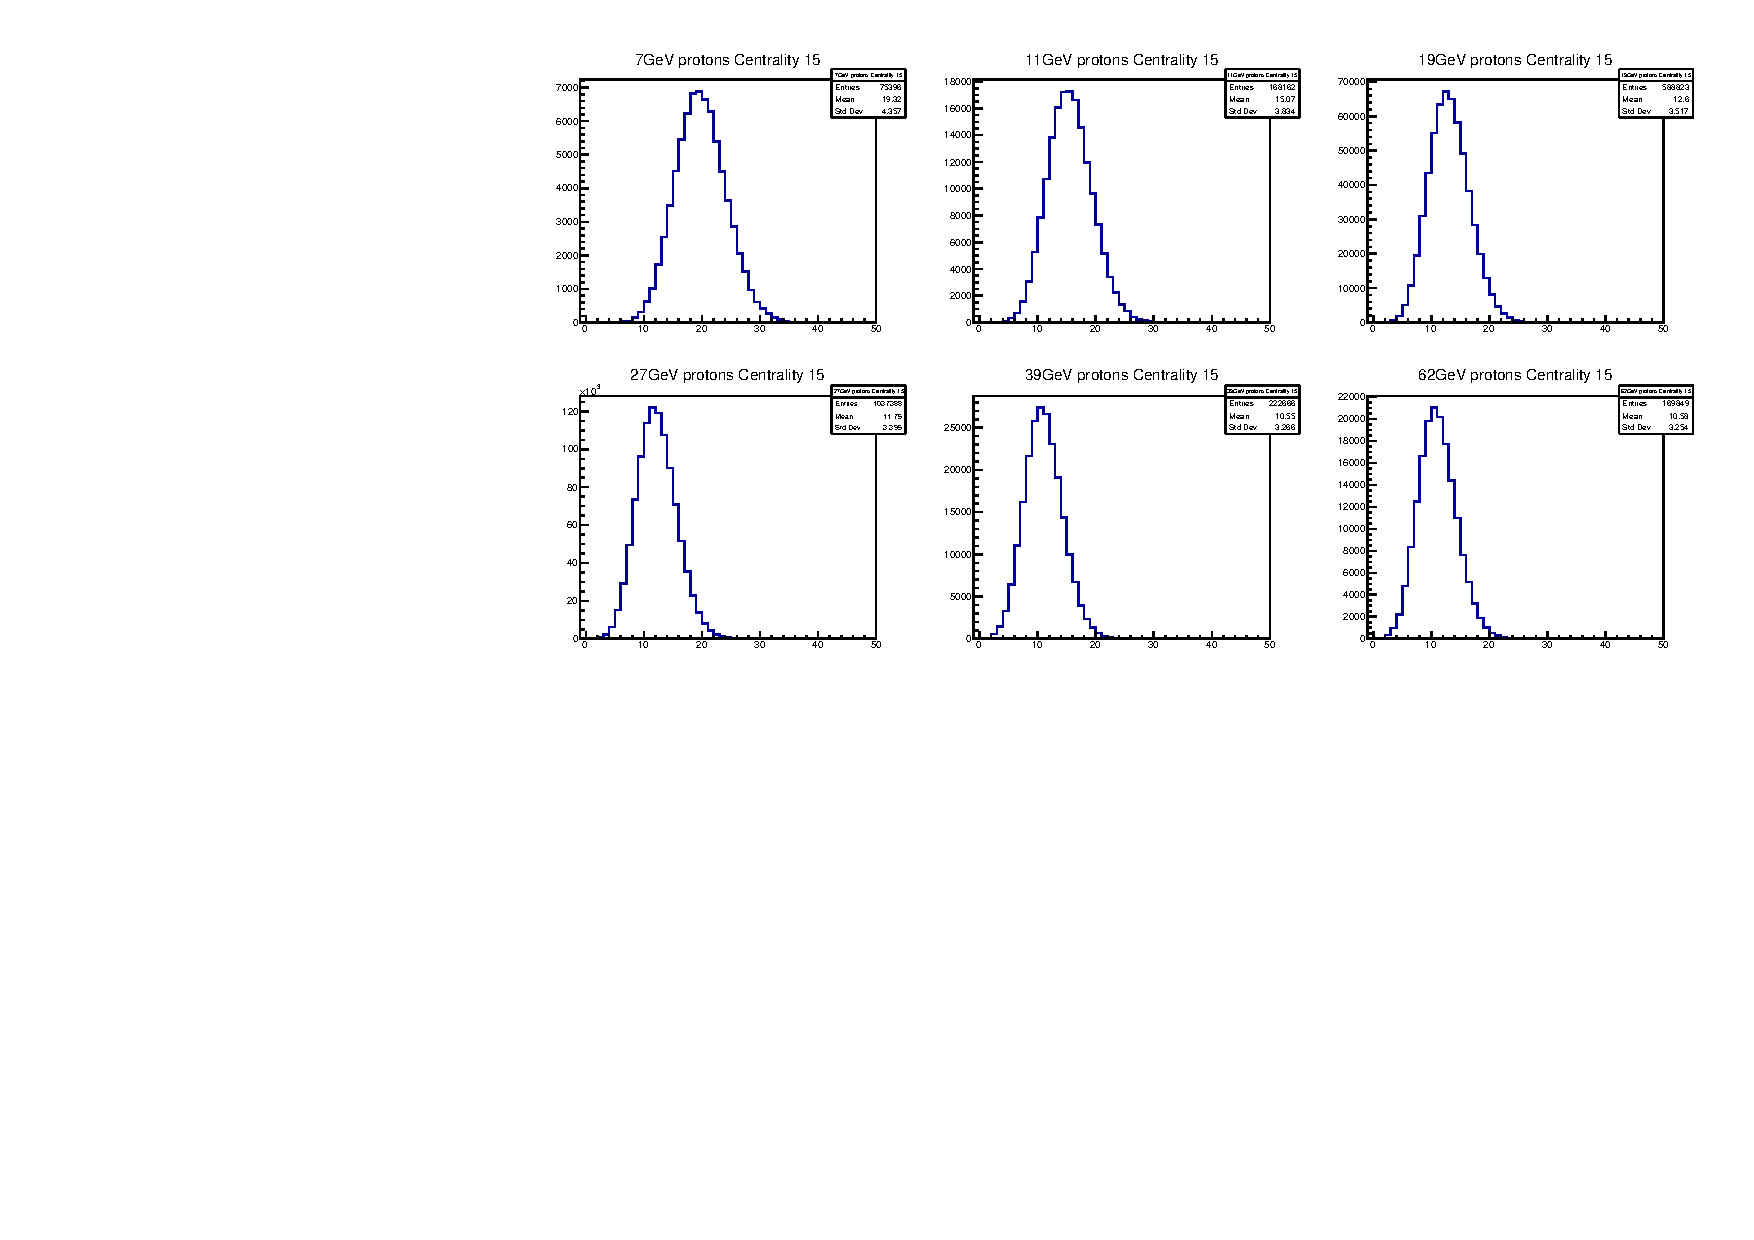
\includegraphics[width=7.4cm]{Distributions/07-08_Proton_Dist.pdf}
}
\end{center}
\begin{center}
\makebox[0cm]{
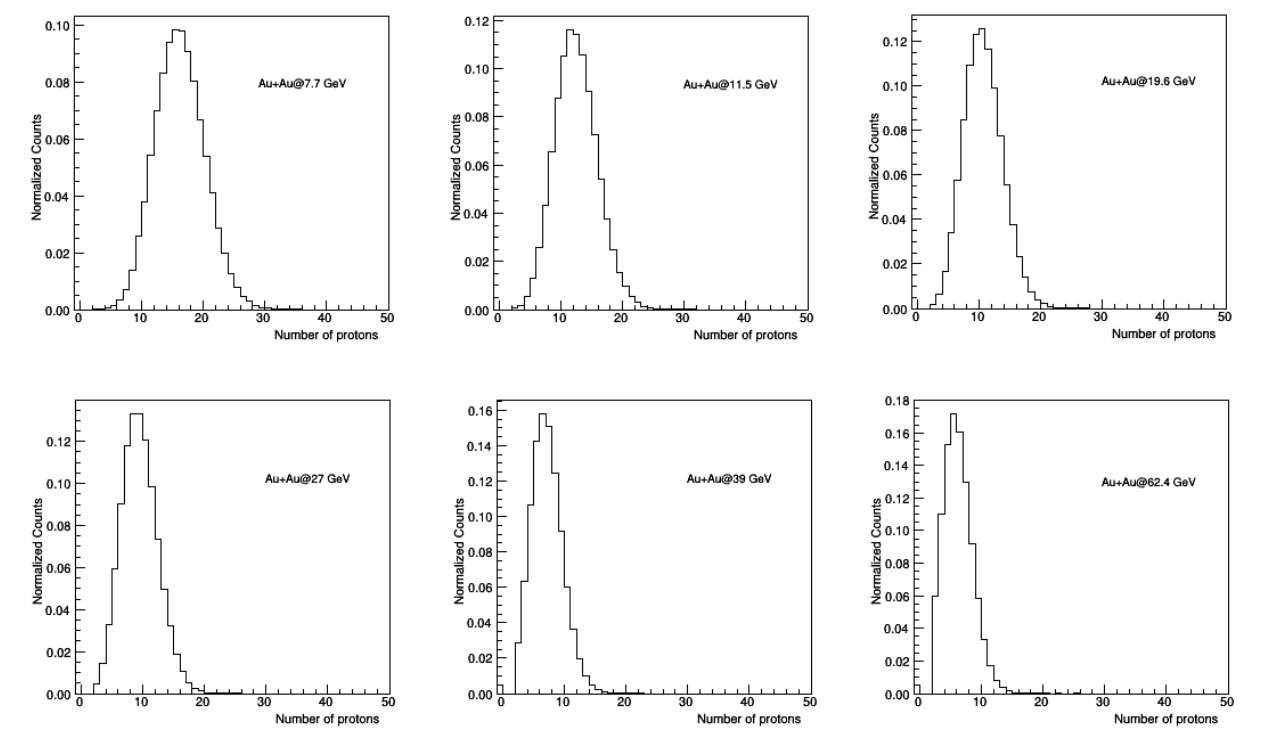
\includegraphics[width=7.4cm]{Distributions/07-05_Proton_Dist_Thesis.png}
}
\end{center}

\end{frame}


\begin{frame}{Proton Distribution Comparison (07-05 top, 07-08 bottom)}

\begin{center}
\makebox[0cm]{
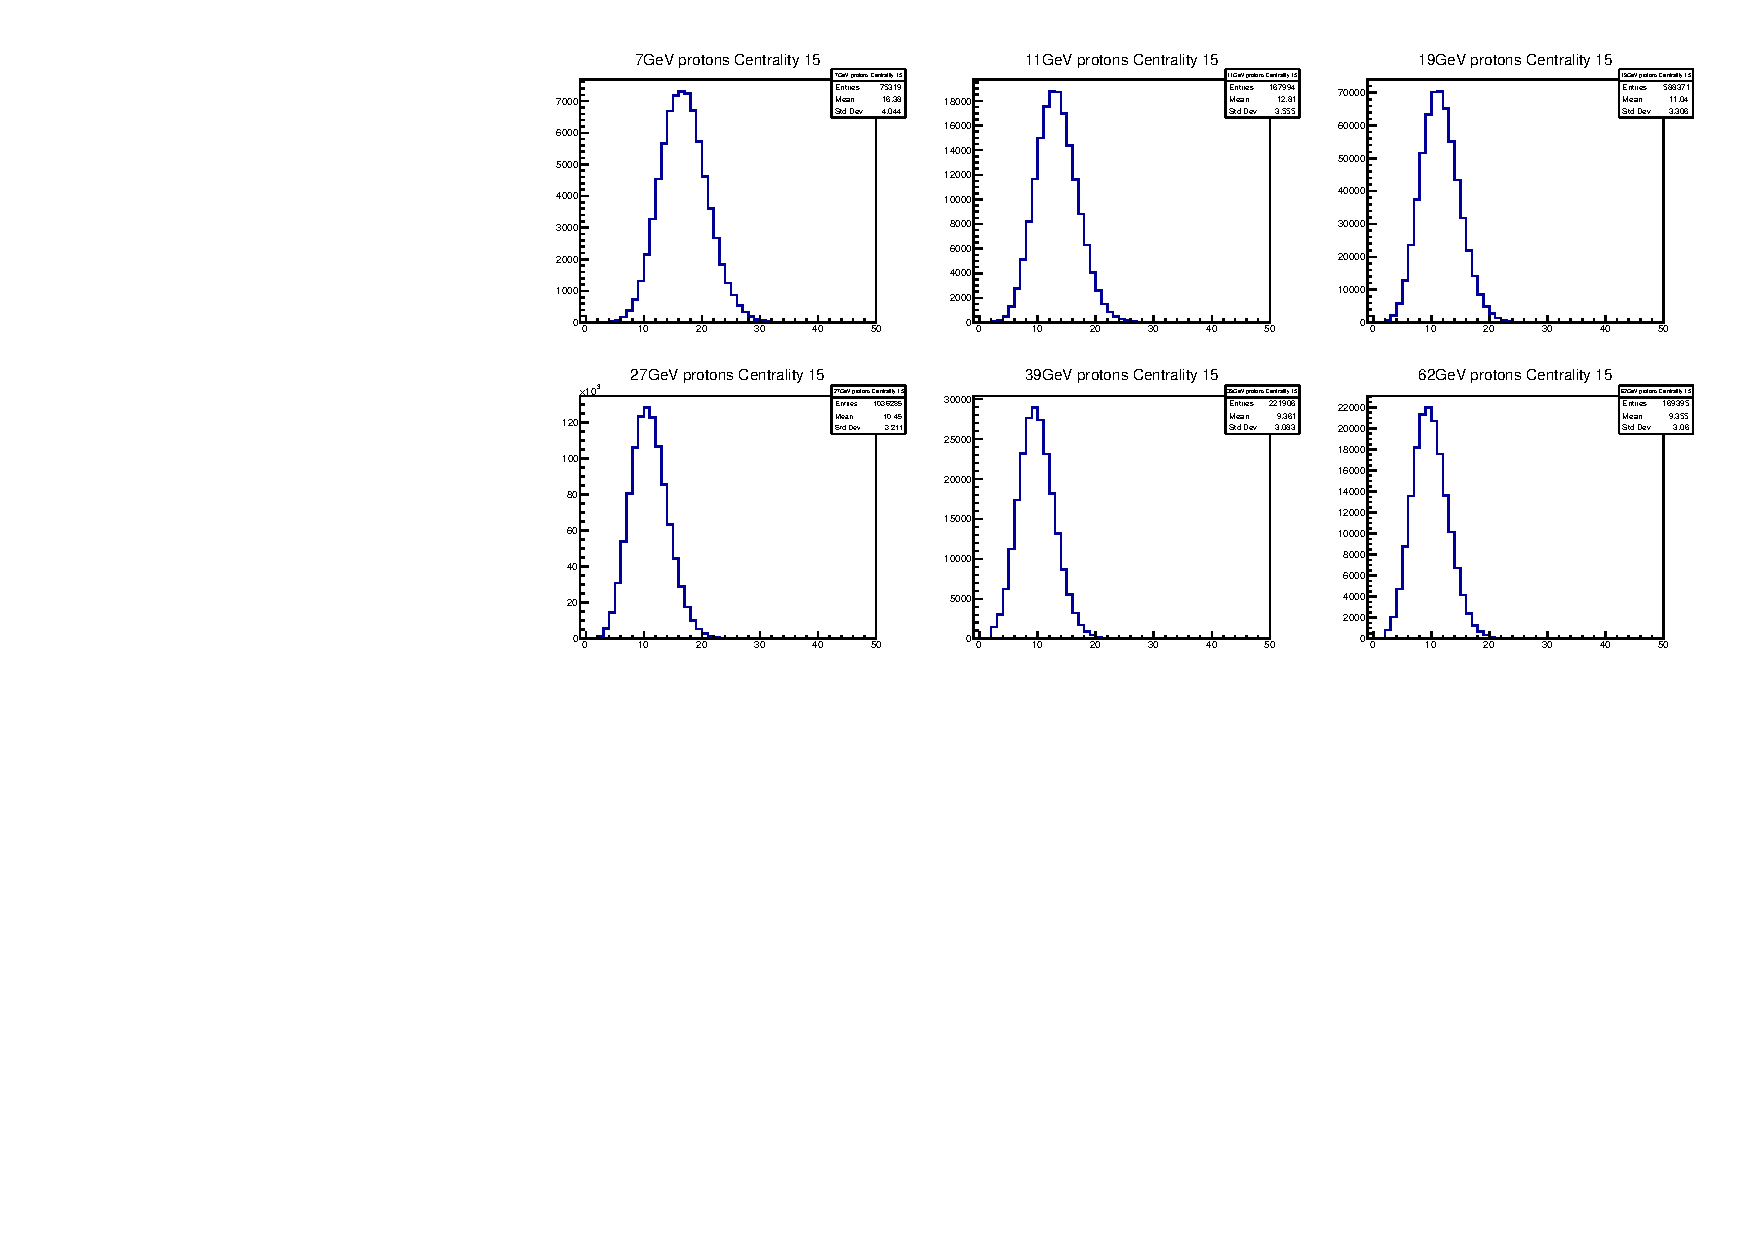
\includegraphics[width=7.4cm]{Distributions/07-05_Proton_Dist.pdf}
}
\end{center}
\begin{center}
\makebox[0cm]{
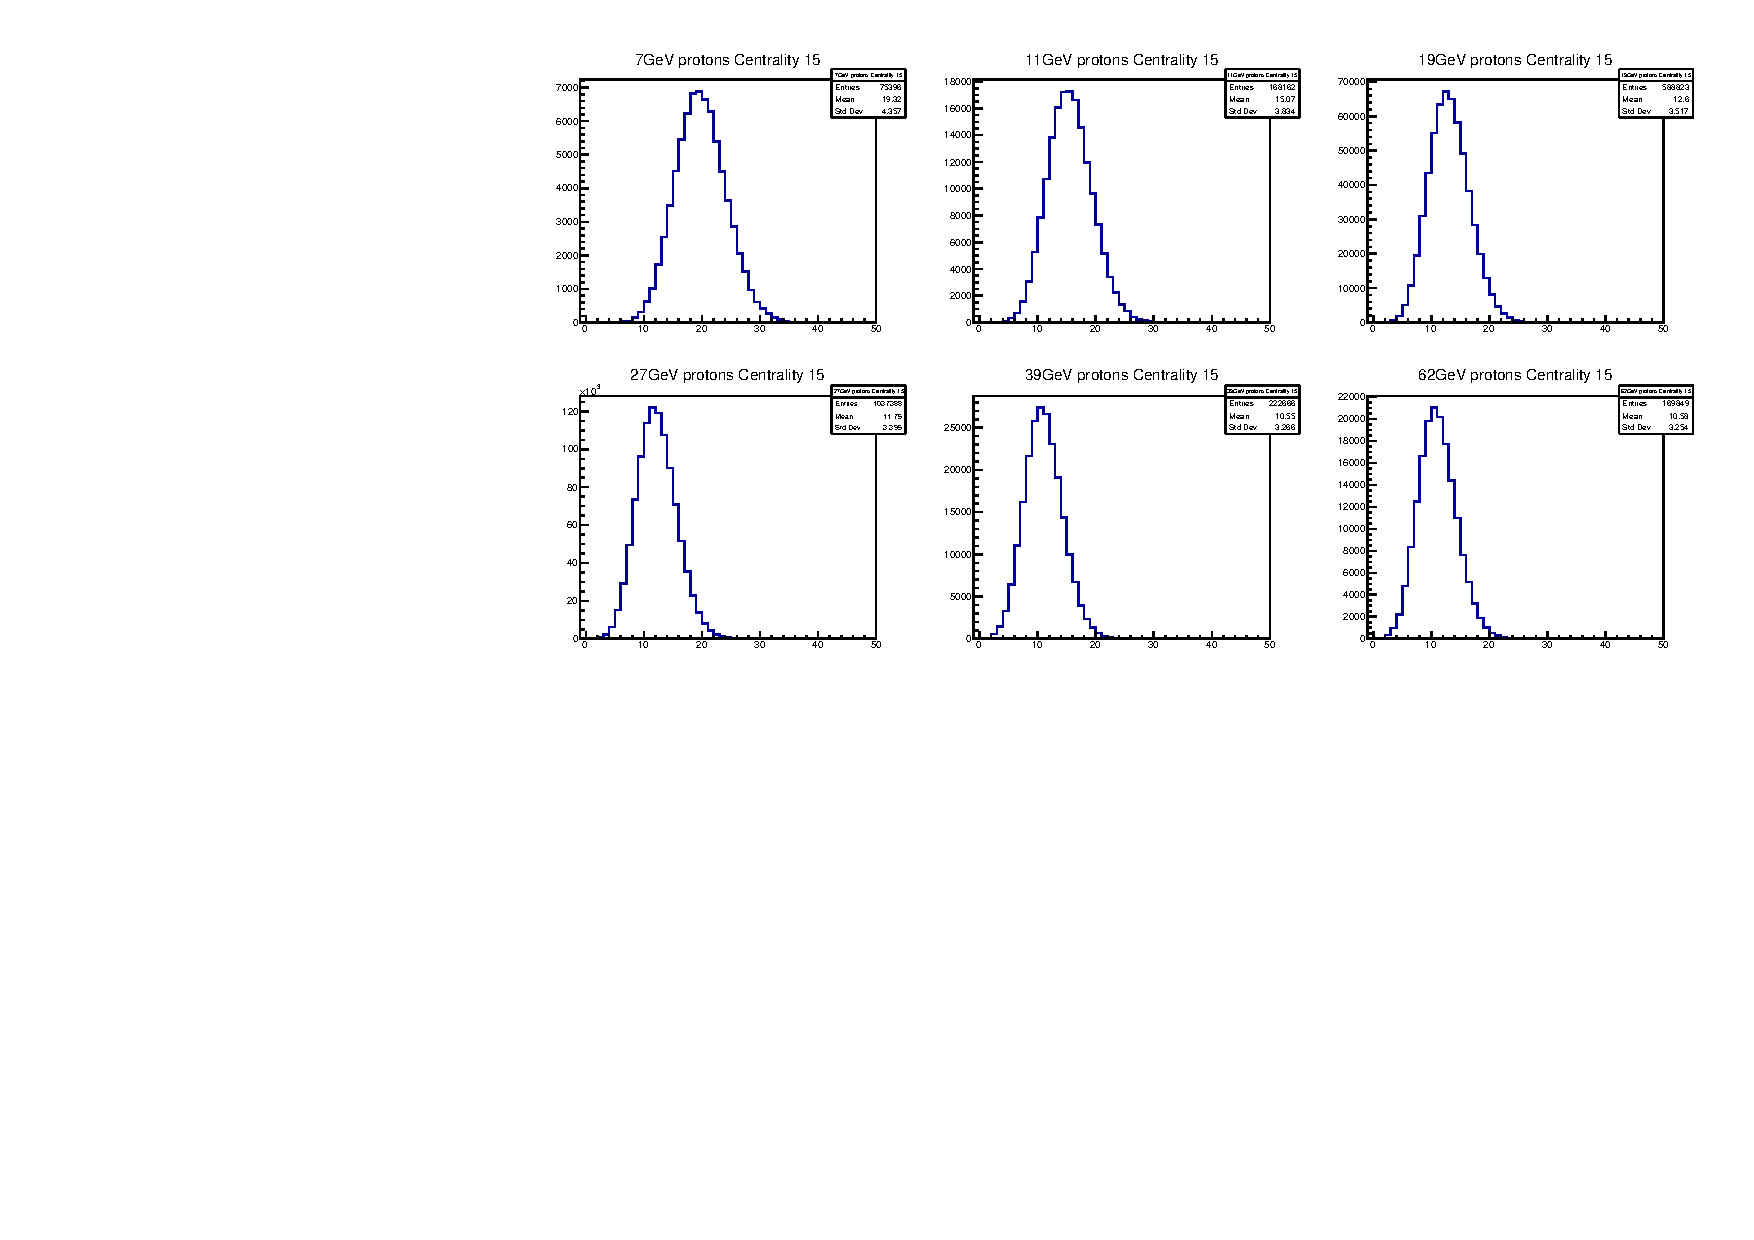
\includegraphics[width=7.4cm]{Distributions/07-08_Proton_Dist.pdf}
}
\end{center}

\end{frame}


\section{Ratio Distribution Comparison}

\begin{frame}{Ratio Distribution Comparison (07-08 top, thesis bottom)}

\begin{center}
\makebox[0cm]{
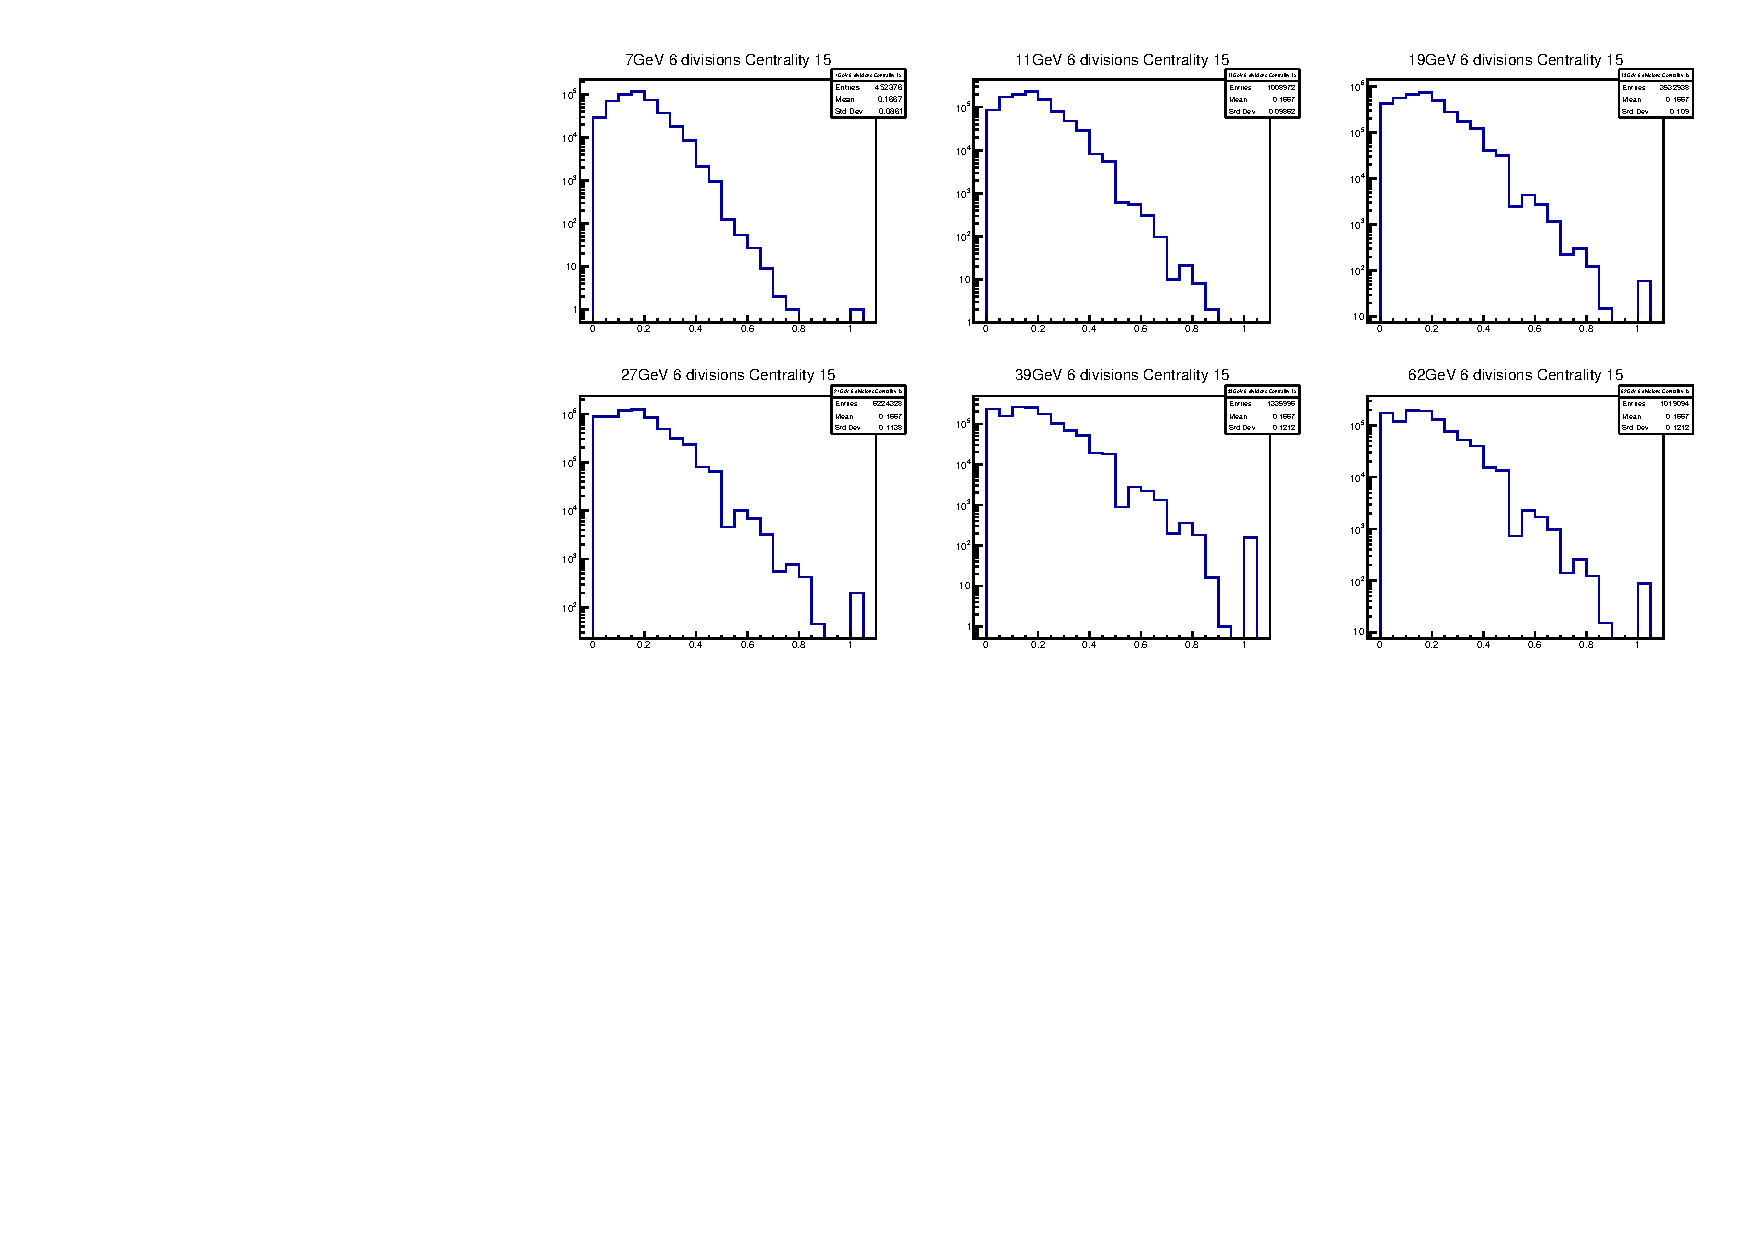
\includegraphics[width=7.1cm]{Distributions/07-08_Ratio_Dist.pdf}
}
\end{center}
\begin{center}
\makebox[0cm]{
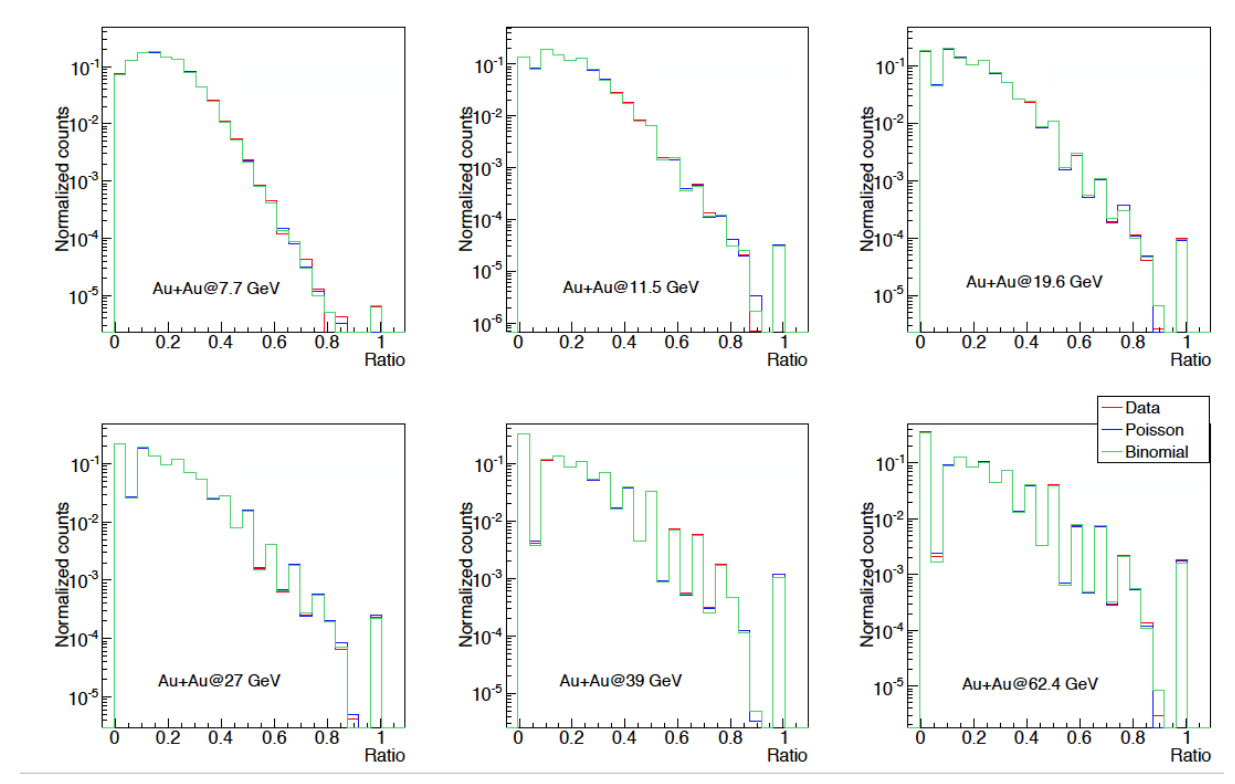
\includegraphics[width=7.1cm]{Distributions/07-05_Ratio_Dists_Thesis.png}
}
\end{center}

\end{frame}

\begin{frame}{Ratio Distribution Comparison (07-05 top, 07-08 bottom)}

\begin{center}
\makebox[0cm]{
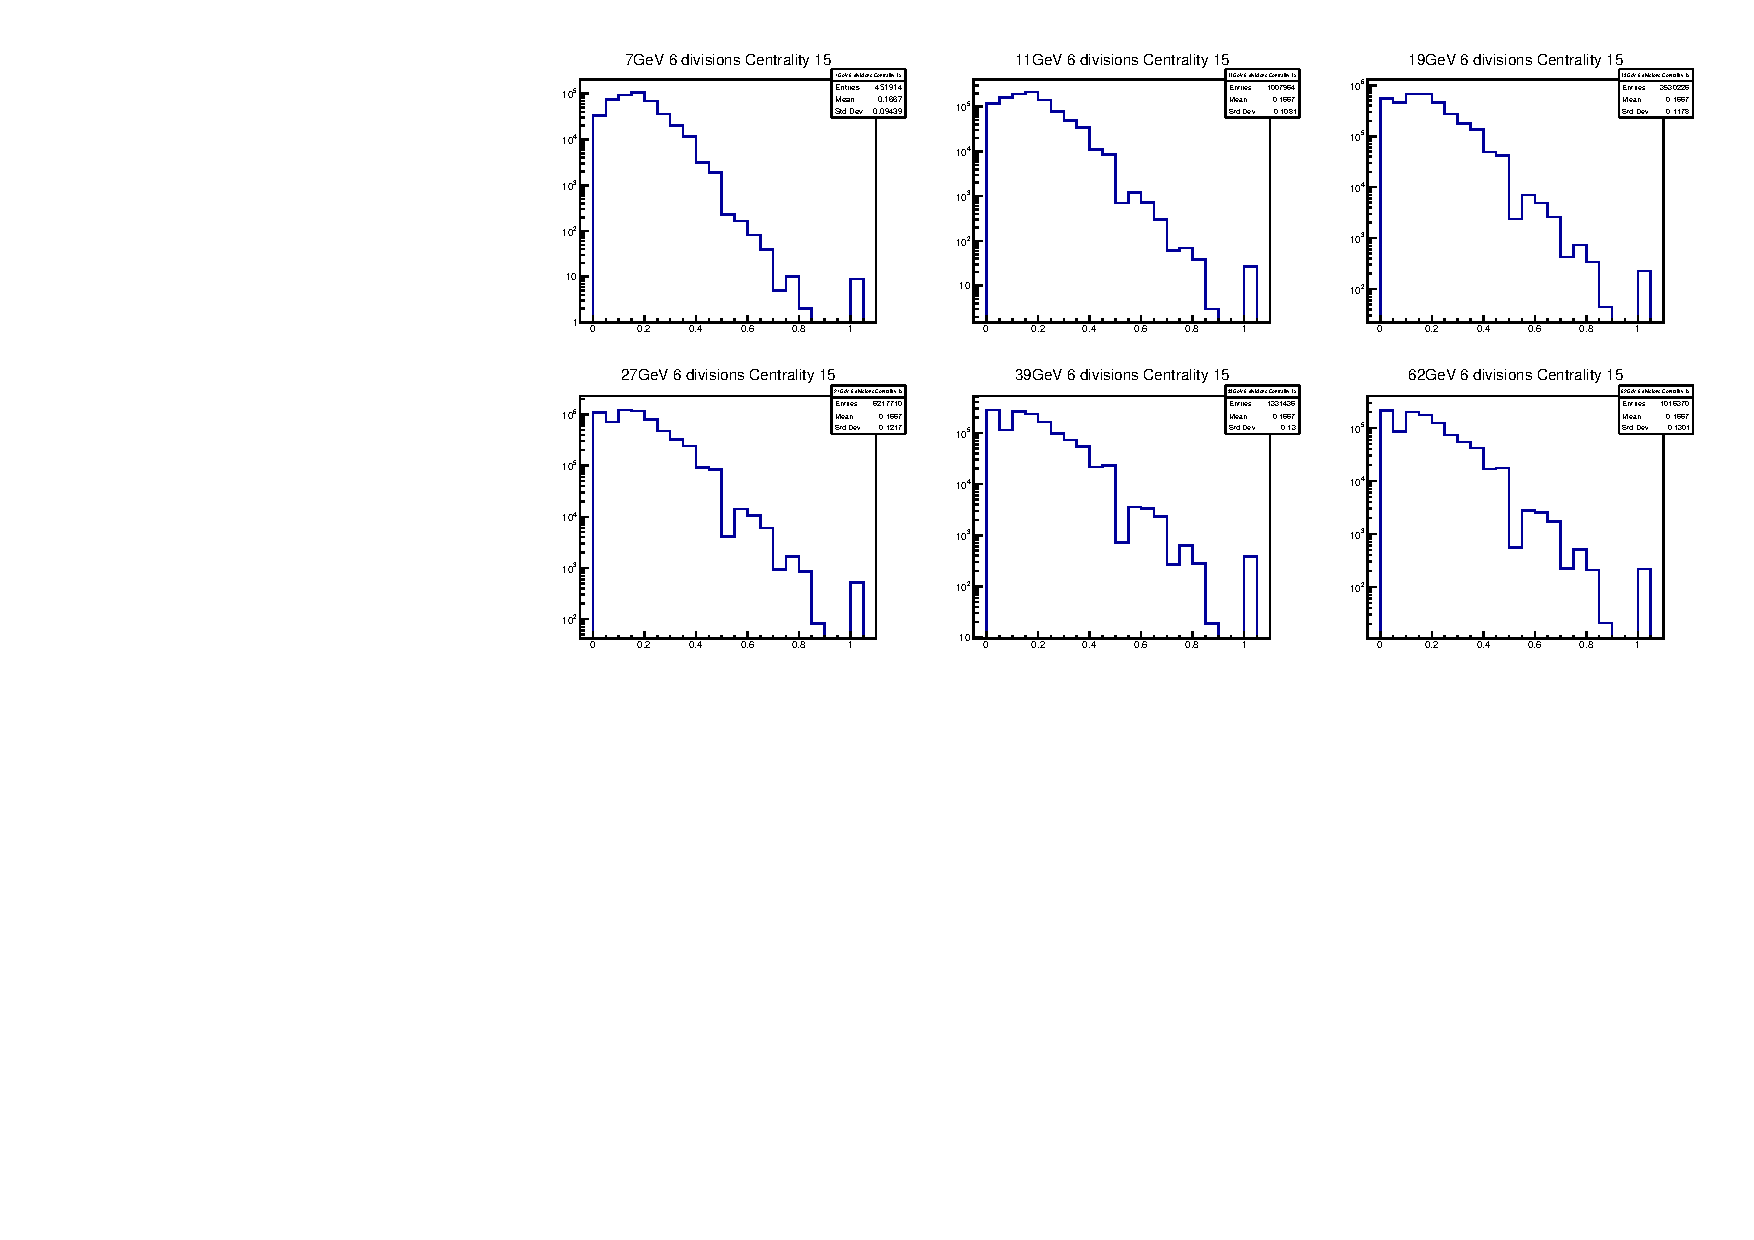
\includegraphics[width=7.1cm]{Distributions/07-05_Ratio_Dist.pdf}
}
\end{center}
\begin{center}
\makebox[0cm]{
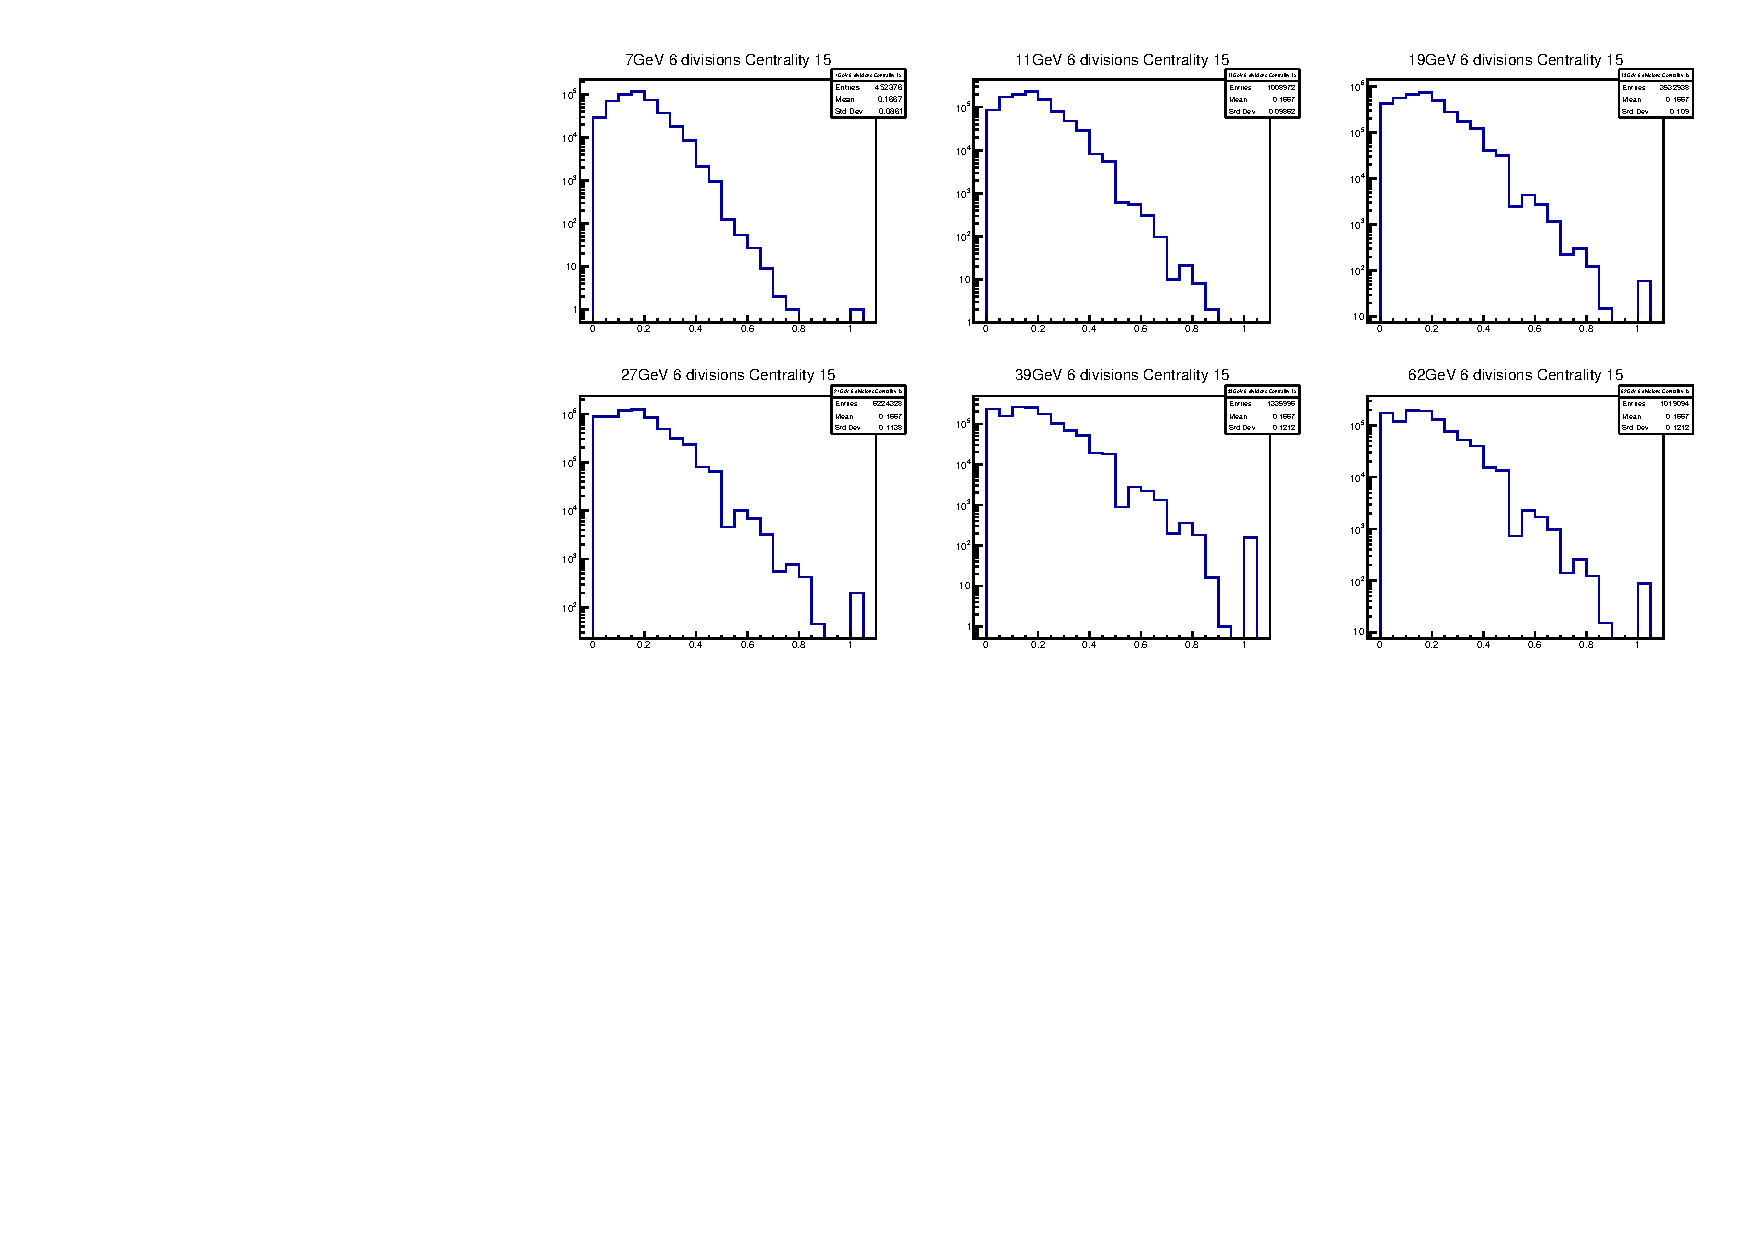
\includegraphics[width=7.1cm]{Distributions/07-08_Ratio_Dist.pdf}
}
\end{center}

\end{frame}

\section{Tree Cuts}

\begin{frame}{Tree Cuts}
"Loose" cuts made on HPSS data when creating trees. \newline \newline \newline
\subsection{Event Level}
Event Level:
	\begin{itemize}
		\item Good runs
		\item $|v_{x}| > 100nm$ or $|v_{y}| > 100nm$ or $|v_{z}| > 100nm$
		\item Good triggers
		\item Primary Vertex z
		\begin{itemize}
		    \item $ < 30cm$
		    \item $ < 50cm$ for 7 GeV
		\end{itemize}
		\item Primary Vertex radial distance $< 2cm$
		\item VPD z within $3cm$ of Primary Vertex z for 39 and 62 GeV
	\end{itemize}
\end{frame}

\begin{frame}{Tree Cuts}
\subsection{Track Level}
Track Level:
    \begin{itemize}
        \item $0.52 <$ nHitsFit / nHitsPossible $< 1.05$ 
        \item nHitsDedx $> 5$
        \item nHitsFit $> 20$
        \item charge $= \pm 1$
        \item p $>0.15$
        \item $-2.2 <$ nSigmaProton $< 2.2$
            \begin{itemize}
                \item For 27GeV $-1 <$ nSigmaProton $< 1$
            \end{itemize}
        \item $-0.6 < \eta < 0.6$
        \item $0 < $ dca $<2.5$
        \item $0.3 <$ pt $< 2.5$
    \end{itemize}

\end{frame}

\section{Analysis Cuts}

\begin{frame}{Analysis Cuts}
Tighter cuts made on tree data when creating ratio observable.
\newline \newline \newline
\subsection{Event Level}
Event Level:
	\begin{itemize}
		\item Good runs
		\item 2 or more good protons for the event.
		\item min slope $<$ btof mult $/$ ref mult $<$ max slope
	\end{itemize}
\end{frame}

\begin{frame}{Analysis Cuts}
\subsection{Track Level}
Track Level:
    \begin{itemize}
        \item pt $< 2.0$
        \item charge $ = 1$
        \item $-0.5 < \eta < -0.5$
        \item $-2.0 < $ nSigmaProton $ < 2.0$
        \item $0.0 <$ dca $< 1.0$
        \item $0.8 < m^2 < 1.0$
            \begin{itemize}
                \item Only if $0.8 <$ pt $< 2.0$ and $\beta > 0$, otherwise keep track
            \end{itemize}
    \end{itemize}
    
\end{frame}

\section{Tree Data Stored}

\begin{frame}{Tree Data Stored}

Event Data:
\begin{itemize}
    \item primaryVertexPosition x,y,z
    \item refMult, refMult2
    \item run number
    \item btofTrayMultiplicity
\end{itemize}
\vspace{1cm}
Track Data:
\begin{itemize}
    \item p, pt, beta
    \item phi, eta
    \item dca
    \item nSigmaProton
    \item charge
\end{itemize}
    
\end{frame}

\section{Btof slope}

\begin{frame}{Btof slope}

\begin{center}
    \begin{tabular}{ c c c }
    Energy & Slope Minimum & Slope Maximum \\
    7 & 2.3309 & 4.36076 \\
    11 & 2.26667 & 4.30469 \\
    14 & 2.80052 & 4.73481 \\
    19 & 2.57482 & 3.736 \\
    27 & 2.7533 & 3.99761 \\
    39 & 3.24125 & 4.8092 \\
    62 & 4.85117 & 6.33216 \\
    200 & 5.87363 & 7.65642
    \end{tabular}
\end{center}
    
\end{frame}


\begin{frame}{RefMult2 Definition}

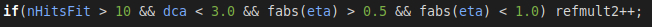
\includegraphics[width = \textwidth]{RefMult2/def.png}
\begin{center}
\makebox[0cm]{
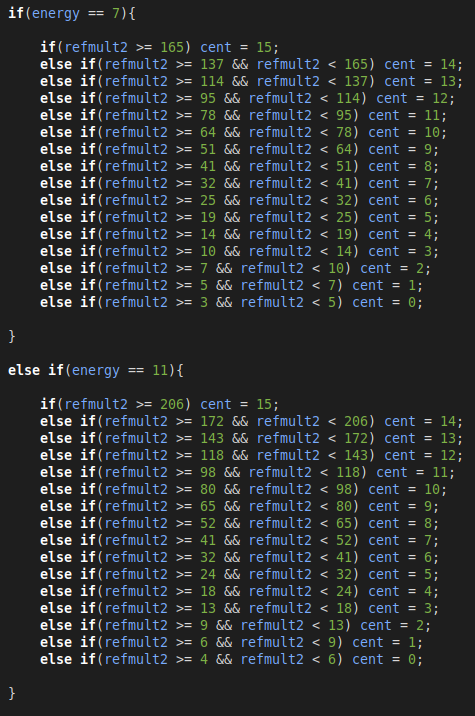
\includegraphics[width=4.2cm]{RefMult2/7-11.png}
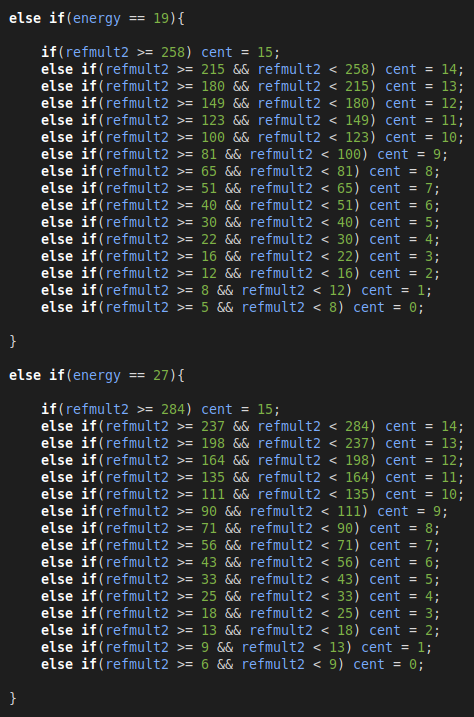
\includegraphics[width=4.2cm]{RefMult2/19-27.png}
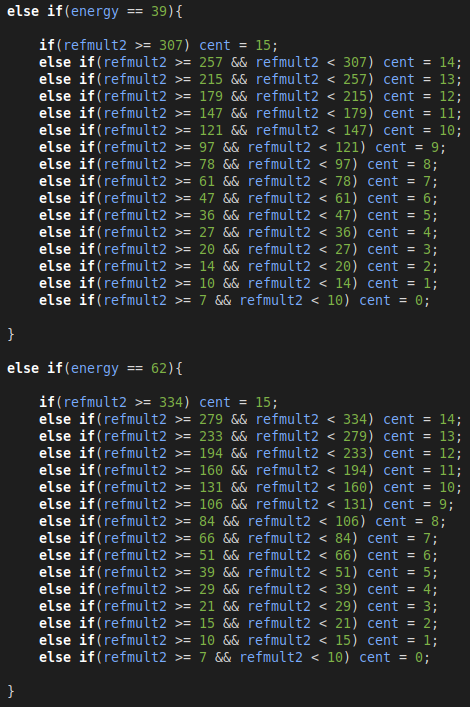
\includegraphics[width=4.2cm]{RefMult2/39-62.png}
}
\end{center}
    
\end{frame}

\end{document}